\chapter{Presentation, Analysis and Interpretation of Data}
\chaptermark{Presentation, Analysis and Interpretation}
	This chapter details the functionalities of the developed system, including its user interface design. Moreover, the system answers the optimal shelter location-allocation for Calumpit. It also presents the evaluation results gathered from the LGU and IT experts, assessing the system’s acceptability and alignment with local needs.

\section{The Developed System}
	The researchers and developers of this thesis developed a decision support system to optimize shelter location allocation since there was a lack of system development. Identifying the most optimal shelter facility for a community is the system's main function. Specifically, it has five key features that let users completely modify the input parameters, and output processing. 


\subsection{Data Modification}
	The process of creating, updating, or deleting data within the system to maintain accuracy and relevance. This ensures that all records are up-to-date and properly managed so they can effectively be used for shelter allocation.
	
	\begin{figure}[h!]
		\caption{Dashboard}
		\centering
		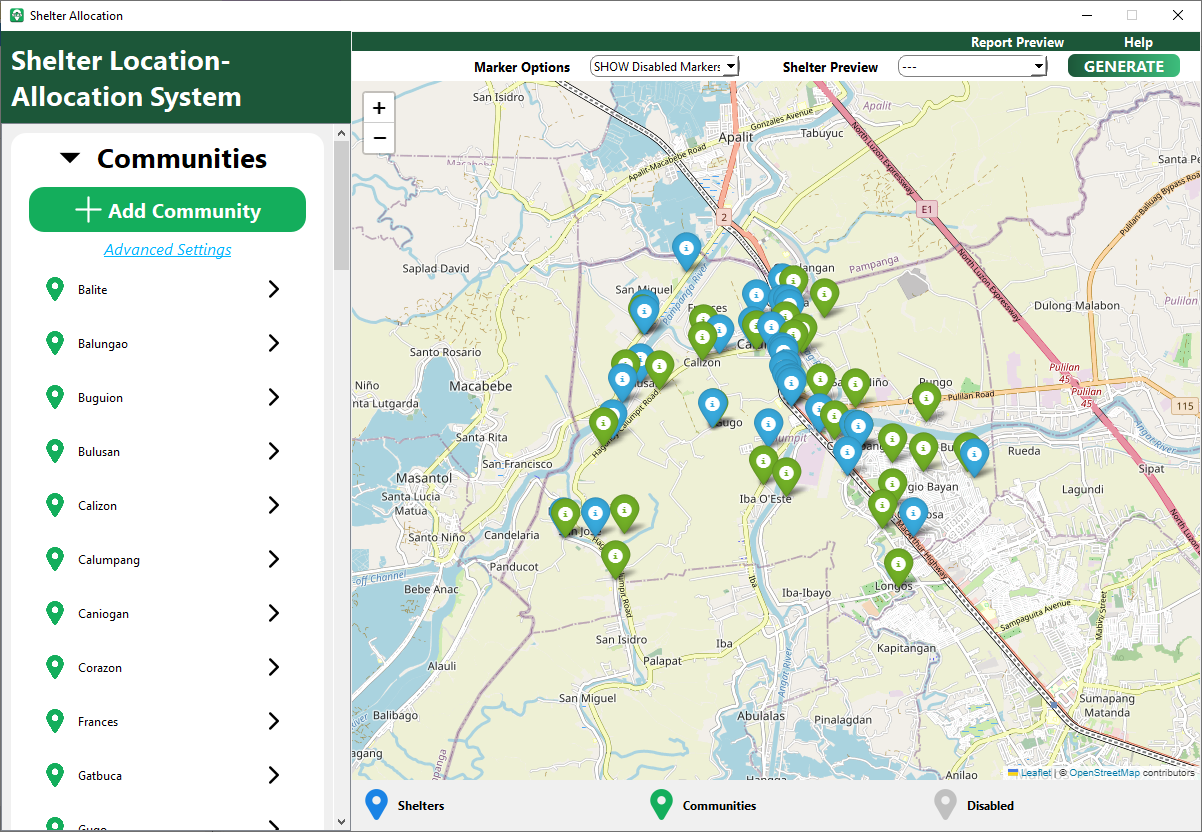
\includegraphics[width=4.5in]{Chapter 4/dashboard}
		\label{db}
	\end{figure}
	The dashboard provides an overview of a list of shelters and communities as shown in figure \ref{db}. It also displays a map where shelters and communities are pinned. Users can see whether a shelter is active or inactive. Additionally, the user can manipulate the map to filter and display only active shelter as well as shelters that are built, partially built, damaged, empty lot, and resistance to flood, typhoon, and earthquake
	
	\begin{figure}[h!]
		\caption{Community Management}
		\centering
		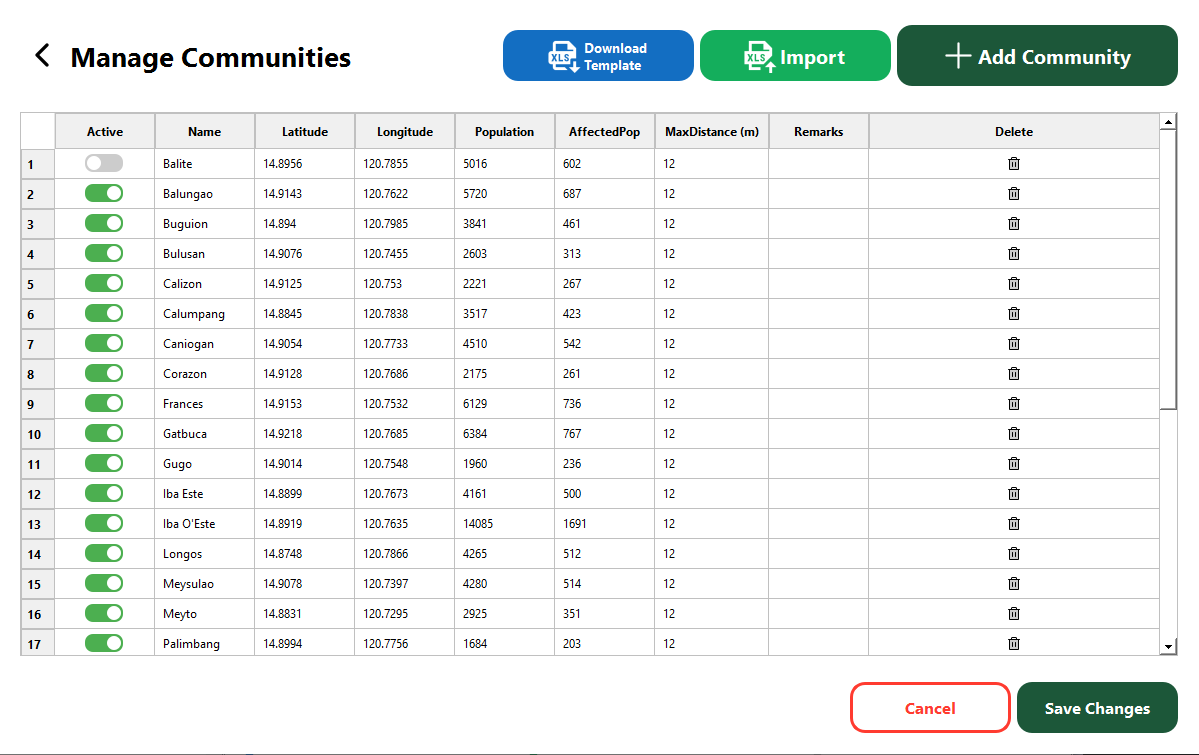
\includegraphics[width=4.5in]{Chapter 4/commadvanced}
		\label{commMan}
	\end{figure}
	Community management module manages the recorded details of barangays as shown in figure \ref{commMan}. It displays whether a barangay is active or inactive, along with its latitude, longitude, population, affected population, maximum distance, remarks, and a delete button. Users can also add new communities, download a template to ensure correct formatting when importing data, and manage barangay-related information efficiently.
	
	\begin{figure}[h!]
		\caption{Shelter Management}
		\centering
		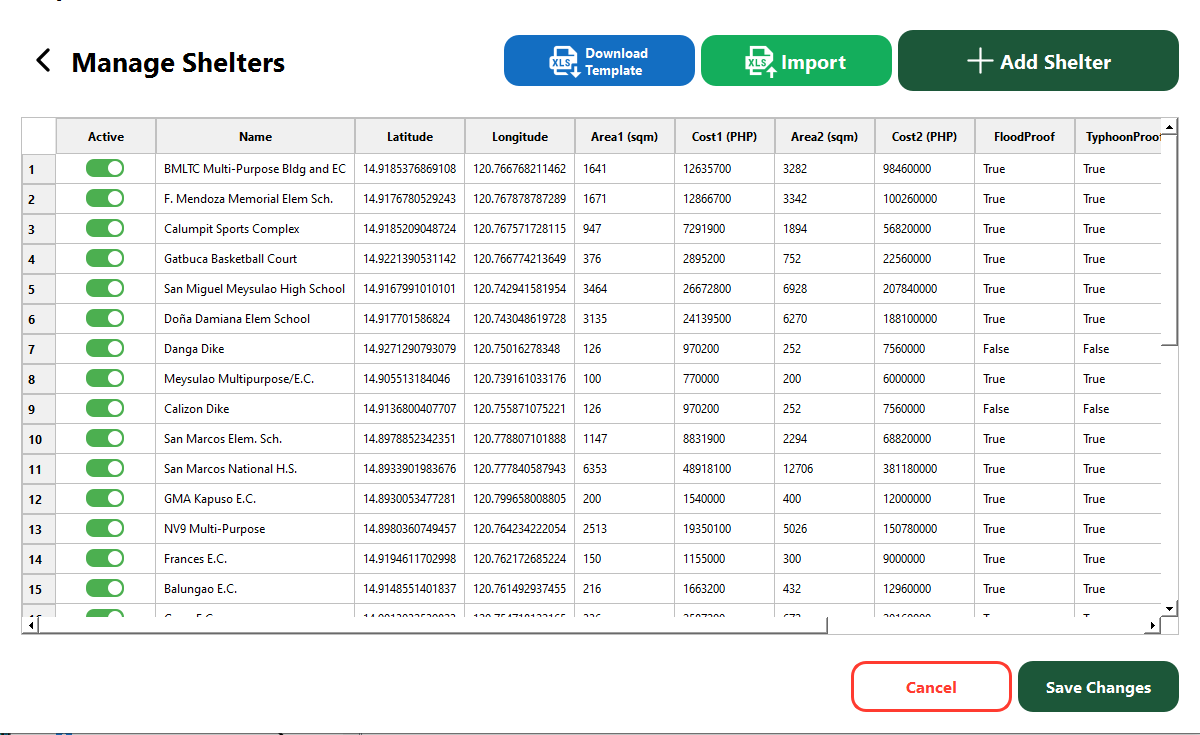
\includegraphics[width=4.5in]{Chapter 4/sheladvanced}
		\label{shelMan}
	\end{figure}
	The shelter management module, as shown in figure \ref{shelMan}, is similar to community management but includes different data fields. It contains information such as the shelter’s name, latitude, longitude, and classification as a Level 1 or Level 2 shelter. The module also tracks the cost of construction and maintenance for each level. Additionally, it indicates whether the shelter is resistant to floods, typhoons, and earthquakes. Users can also view the shelter’s status – whether it is built, partially built, damaged, or an empty lot.
	
\subsection{Model Modification}
	This concerns the parameters to be used in the model that may be modified for a more ideal setup depending on the preferences of the user. The parameters that may be changed here include the area per individual based on meters squared, the max number of level 2 shelters and shelters in general, the weights for both distance and cost, the number of generations, the number of populations in a generation, and the mutation rate. Measures are put in place to prevent entering of wrong values in these parameters such as letters or negative numbers. 
	
	\begin{figure}[h!]
		\caption{Model Parameter Settings}
		\centering
		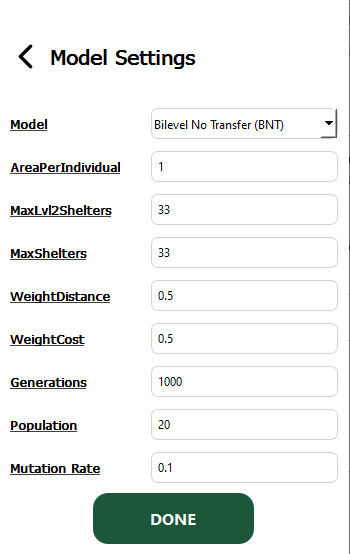
\includegraphics[width=2.5in]{Chapter 4/modelsettings}
		\label{modelSet}
	\end{figure}
	These factors impact the time taken to simulate data as well as the efficiency of the simulation, it is recommended to keep the parameters at default values unless the user is knowledgeable about the model or the system. These parameters are modified in the Model Parameter Settings module as shown in figure \ref{modelSet}, which may be accessed from the Solve Settings module by clicking Advanced Settings below Model.
	
	
\subsection{Data Simulation}
	This pertains to solving the model by running the Genetic Algorithm, which determines the most optimal shelter location allocation. As the core functionality of the system, it processes input data of communities and shelters, applies defined model parameters, then generates and displays the best allocation of the municipality.
	
	\begin{figure}[h!]
		\caption{Progress Dialog}
		\centering
		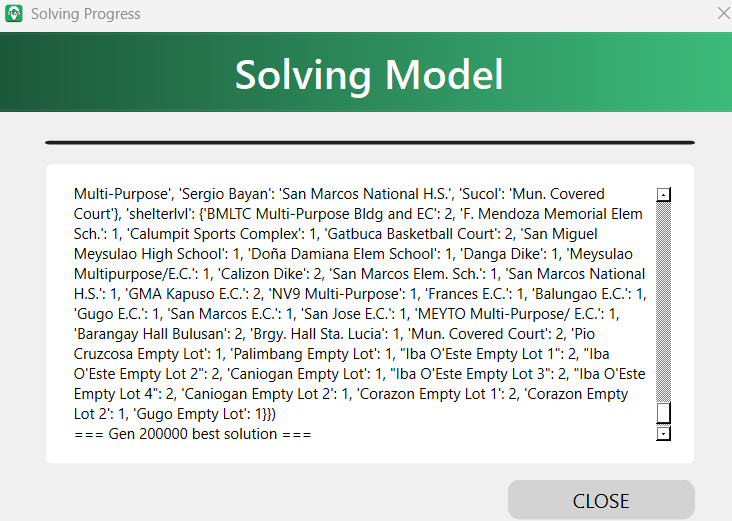
\includegraphics[width=3.5in]{Chapter 4/progress}
		\label{solveProg}
	\end{figure}
	Progress dialog as shown in figure \ref{solveProg} provides real-time logs and tracks the progress of the simulation. The process starts by computing the distances between each community and each shelter using a Python library, OSMnx. Once the distances are calculated, the system proceeds with the Genetic Algorithm to optimize the allocation. Users also have the option to cancel the process at any time.
	
	\begin{figure}[h!]
		\caption{Report Dialog}
		\centering
		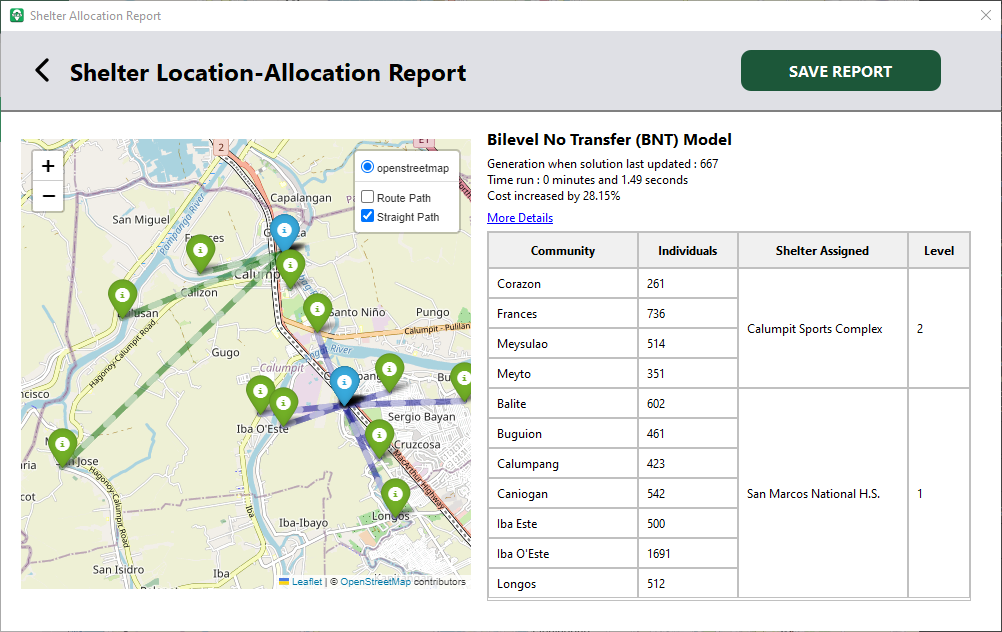
\includegraphics[width=4.5in]{Chapter 4/alloc report}
		\label{shelAllocRep}
	\end{figure}
	After the solving process is completed, report dialog appears displaying the final allocation results as shown in figure \ref{shelAllocRep}. It shows which communities are assigned to shelters, and displays the paths they can take on a map. This helps users analyze the feasibility and efficiency of the allocation.
	
	The Genetic Algorithm is implemented from scratch using Python, ensuring full control over its functionality and optimization process. The main functions in the code include fitness calculation, constraint enforcement, and the implementation of selection, mutation, and crossover.
	
	Appendix \ref{objValCode} details the fitness calculation, which represents the model's objective value. The first loop calculates the total distance, while the second loop determines the cost based on the level of the opened shelters.
	
	Appendices \ref{maxdistCode}, \ref{capCode}, \ref{maxshelCode}, and \ref{maxl2shelCode} implement the constraint functions, adding penalties to the objective value when violated. These constraints include maximum distance constraint, initial capacity constraint, maximum number of level 2 shelters that can be constructed/allocated, maximum number of shelters that can be constructed/allocated. Since the implemented Genetic Algorithm operates on integers, the constraints ensuring that each community is assigned only one shelter and one level are already satisfied.
	
\subsection{Shelter Tagging}
	This concerns the classification of shelters based on both structural resilience and current condition, ensuring shelters are appropriately assigned to communities based on availability, cost, and risk levels. Shelters are categorized in both resistance capabilities and status; resistance capabilities include flood-resistant, typhoon-resistant, and earthquake-resistant, and are not mutually exclusive to one another, for example, a shelter can be both flood and typhoon resistant. In terms of status, shelters can be built, partially built, damaged, and empty lots, each with varying costs depending on maintenance and construction.
	
	\begin{figure}[h!]
		\caption{Solve Settings}
		\centering
		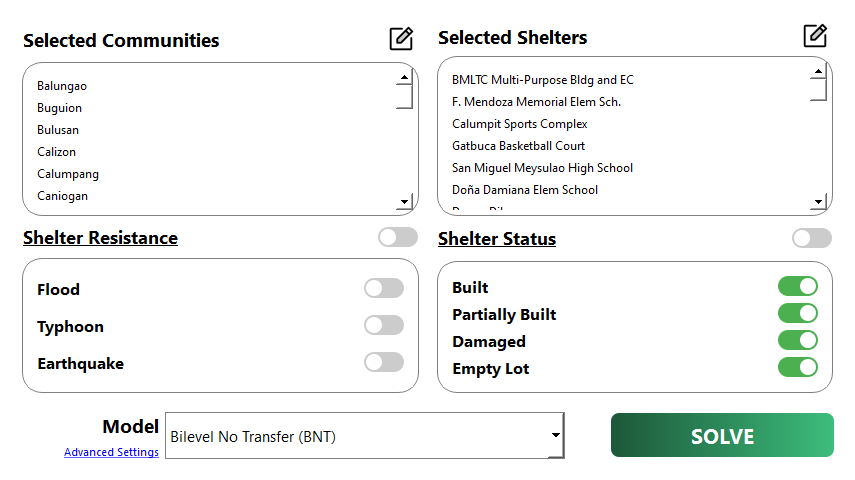
\includegraphics[width=3.5in]{Chapter 4/solvesettings}
		\label{solveSet}
	\end{figure}
	Selecting shelters with specific resistances and statuses in mind is done in the Solve Settings module as shown in figure \ref{solveSet}, where selecting or deselecting a specific resistance will remove shelters that do not meet the criteria from the data simulation. This ensures users will not assign communities to shelters that are not suited to the situation. Users may also check the status and resistances of a specific shelter in either the dashboard module by selecting a shelter, or in the shelter advanced settings, displaying all shelters’ statuses.
	

\subsection{Report Protection}
	To maintain confidentiality and prevent the unauthorized modification of reports, a security mechanism has been implemented in the system. This module includes password authentication, report encryption and identification of the creator of a report based on device-specific attributes.
	
	\begin{figure}[h!]
		\caption{Input Password Popup}
		\centering
		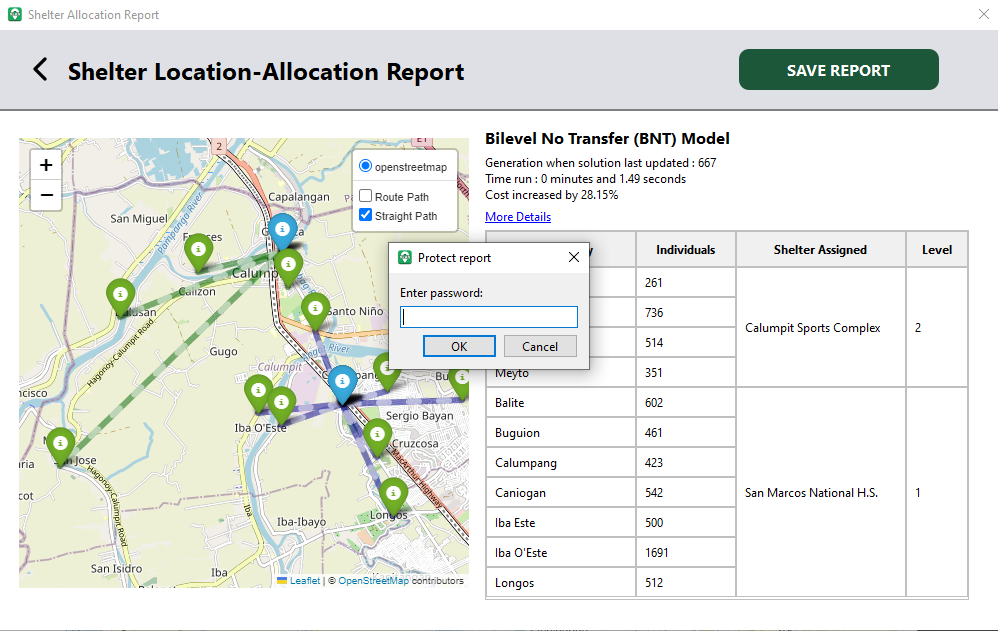
\includegraphics[width=4.5in]{Chapter 4/alloc report pass}
		\label{passPop}
	\end{figure}
	Upon finishing data simulation, the generated report may be saved in an excel format, and gives users the option to add password protection to the file through a popup as shown in figure \ref{passPop}. This ensures only intended users may access the report, the generated excel file itself is also read-only, without the ability to modify the data without authorization. The protected file was encrypted using a Python library, MSoffcrypto.
	
	The excel file also contains identification of the creator of the report, containing three device-specific identifiers, the IP address or the location of the user’s device, the MAC address or the identifier of the user’s network interface, as well as the name of the device the report was generated in. This information is logged in the password protected excel file, enhancing security and ensuring unauthorized users are logged and tracked. 
	
\section{Generated Shelter Location-Allocation Report}
	This section discusses the process of generating reports for shelter location allocation. The report helps in optimizing shelter assignments for communities based on various parameters and ensuring efficient disaster response. The data used considers only 12\% of the population in each barangay as affected. Additionally, the shelters have a maintenance cost, which are factored into the optimization process.
	
	Table \ref{modelParams} shows the parameters used for the BNT model and the genetic algorithm. Table \ref{calReport} presents the optimized shelter location-allocation results generated by the system. Five shelters were opened and assigned to respective communities. All shelters were opened as Level 1, except for Mun. Covered Court, which was upgraded to Level 2. This suggests that upgrading this shelter is better than opening an additional one.
	
	\begin{table}[h]
		\centering
		\caption{Model Parameters}
		\label{modelParams}
		\begin{tabular}{|c|c|}
			\hline
			\textbf{Parameter} & \textbf{Value} \\ \hline
			Area Per Individual in $m^2$ & 1 \\ 
			Maximum Level 2 Shelters  & 33 \\ 
			Maximum Shelters & 33 \\ 
			Weight Distance & 0.5 \\ 
			Weight Cost & 0.5 \\ 
			Generations & 200000 \\ 
			Population & 100 \\ 
			Mutation Rate & 0.1 \\ \hline
		\end{tabular}
	\end{table}
	
	\begin{table}[h!]
		\centering
		\caption{Generated Shelter Location-Allocation for Calumpit}
		\label{calReport}
		\renewcommand{\arraystretch}{1.2} 
		\resizebox{0.75\columnwidth}{!}{
			\begin{tabular}{|c|c|c|}
				\hline
				\textbf{Community} & \textbf{Shelter Assigned} & \textbf{Level} \\ \hline
				Calizon & \multirow{5}{*}{Doña Damiana Elem School} & \multirow{5}{*}{Level 1} \\ \cline {1-1} 
				Frances & & \\ \cline {1-1} 
				Gatbuca & & \\ \cline {1-1} 
				Meysulao & & \\ \cline {1-1} 
				San Miguel  & & \\ \hline
				Bulusan & \multirow{6}{*}{Mun. Covered Court} & \multirow{6}{*}{Level 2} \\ \cline {1-1} 
				Corazon & & \\ \cline {1-1} 
				Panducot & & \\ \cline {1-1} 
				Poblacion & & \\ \cline {1-1} 
				Santa Lucia & & \\ \cline {1-1} 
				Sucol & & \\ \hline
				Balungao & \multirow{5}{*}{NV9 Multi-Purpose} & \multirow{5}{*}{Level 1} \\ \cline {1-1} 
				Meyto & & \\ \cline {1-1} 
				San Jose & & \\ \cline {1-1} 
				Santo Niño & & \\ \cline {1-1} 
				Sapang Bayan & & \\ \hline
				Caniogan & \multirow{3}{*}{San Marcos Elem. Sch.} & \multirow{3}{*}{Level 1} \\ \cline {1-1} 
				Palimbang & & \\ \cline {1-1} 
				San Marcos & & \\ \hline
				Balite & \multirow{10}{*}{San Marcos National H.S.} & \multirow{10}{*}{Level 1} \\ \cline {1-1} 
				Baguion & & \\ \cline {1-1} 
				Calumpang & & \\ \cline {1-1} 
				Gugo & & \\ \cline {1-1} 
				Iba Este & & \\ \cline {1-1} 
				Iba O'Este & & \\ \cline {1-1} 
				Longos & & \\ \cline {1-1} 
				Pio Cruzcosa & & \\ \cline {1-1} 
				Pungo & & \\ \cline {1-1} 
				Sergio Bayan & & \\ \hline
			\end{tabular}
		}
	\end{table}
	
	\begin{table}[h!]
		\centering
		\caption{Result Details}
		\label{resdetails}
		\begin{tabular}{|c|c|}
			\hline
			\textbf{Item} & \textbf{Value} \\ \hline
			Objective Value & 72034087 \\ 
			Time Run  & 73 minutes and 30.96 seconds \\ 
			Cost of Opened Shelters & 144019600 \\ 
			Generation when solution last updated & 136256 \\ \hline
		\end{tabular}
	\end{table}
	
	\begin{figure}[h!]
		\centering
		\caption{Community to Shelter Paths}
		\begin{subfigure}{0.4\textwidth}
			\caption{Straight Path}
			\centering
			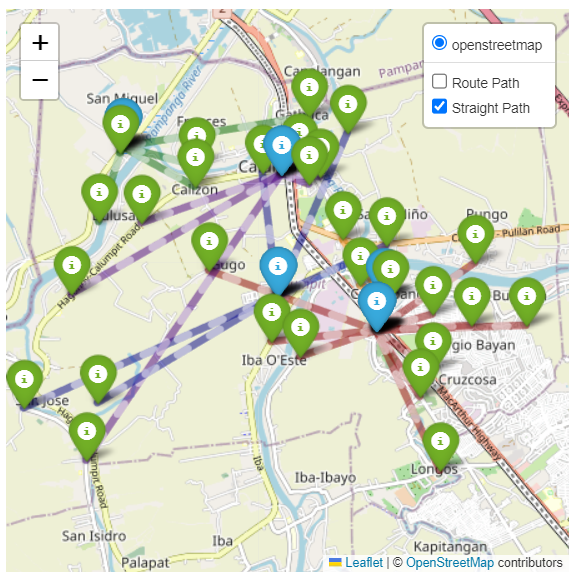
\includegraphics[width=\textwidth]{Chapter 4/straight path}
			\label{straightpath}
		\end{subfigure}
		\hspace{0.5cm}
		\begin{subfigure}{0.4\textwidth}
			\caption{Route Path}
			\centering
			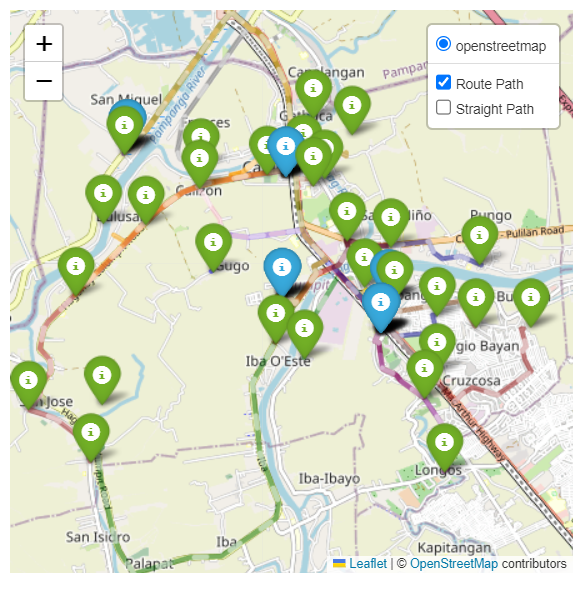
\includegraphics[width=\textwidth]{Chapter 4/route path}
			\label{routepath}
		\end{subfigure}
		
	\end{figure}
	
	 Table \ref{resdetails} shows the details of the result. Note that this report is generated by the system running on Huawei Matebook D15 with processor of Ryzen 7 5700U. The generated report can be downloaded as an Excel file. In the Report Module, a map displays where communities are allocated to their designated shelters. Figure \ref{straightpath} and \ref{routepath} shows the generated map which visualizes the allocation result.
	
\section{System Evaluation}
	The developed system underwent an assessment through survey questionnaires to evaluate its acceptability. The respondents included the target users, specifically the MSWDO and MDRRMO of Calumpit. In addition, IT experts with experience in system development participated in the evaluation to provide technical insights and ensure that the system met quality standards.

\subsection{End-Users}
	The researchers conducted a survey to 23 respondents from the MSWDO and MDRRMO of Calumpit. The survey instrument was based on TAM which consists of four criteria: perceived usefulness, perceived ease of use, attitude towards using, and behavioral intention to use. The gathered data was analyzed to determine the users’ acceptance of the system. 

	\begin{table}[h!]
		\centering
		\caption{Perceived Usefulness Evaluation}
		\label{percuse}
		\renewcommand{\arraystretch}{1.2}
		\begin{tabularx}{\linewidth}{|X|c|c|c|}
			\hline
			\textbf{Statement} & \textbf{Mean} & \textbf{SD} & \textbf{VI} \\ \hline
			Using the system improves my performance in completing tasks such as planning shelter locations for disaster response.
			& 9.35 & 0.71 & Strongly Agree \\ \hline
			The system helps me accomplish choosing shelter locations and assigning communities more quickly.
			& 9.22& 0.80 & Strongly Agree  \\ \hline
			The system increases my productivity.
			& 9.22 & 0.60 & Strongly Agree  \\ \hline
			The system enhances my effectiveness in completing tasks such as in disaster strategic planning.
			& 9.43 & 0.59 & Strongly Agree  \\ \hline
			Overall, I find the system useful in my job.
			& 9.74 & 0.54 & Strongly Agree  \\ \hline
			\textbf{TOTAL MEAN} & \textbf{9.40} & & \textbf{Strongly Agree}  \\ \hline
		\end{tabularx}
	\end{table}
	
	Table \ref{percuse} shows the users’ perceived usefulness of the system. The result shows a total mean score of 9.4, which corresponds to "Strongly Agree," indicating “Highly Acceptable” in terms of perceived usefulness. The standard deviations range from 0.54 to 0.8, implying low variation in the respondents’ answers.
	
	\begin{table}[h!]
		\centering
		\caption{Perceived Ease of Use Evaluation}
		\label{percease}
		\renewcommand{\arraystretch}{1.2}
		\begin{tabularx}{\linewidth}{|X|c|c|c|}
			\hline
			\textbf{Statement} & \textbf{Mean} & \textbf{SD} & \textbf{VI} \\ \hline
			Learning to operate the system is easy for me.
			& 9.39 & 0.58 & Strongly Agree \\ \hline
			The system is easy to use.
			& 9.39 & 0.58 & Strongly Agree \\ \hline
			My interaction with the system is clear and understandable.
			& 9.43 & 0.66 & Strongly Agree \\ \hline
			I find it easy to become skillful at using the system.
			& 9.61 & 0.58 & Strongly Agree \\ \hline
			I find the system easy to operate.
			& 9.52 & 0.59 & Strongly Agree \\ \hline
			\textbf{TOTAL MEAN} & \textbf{9.47} & & \textbf{Strongly Agree} \\ \hline
		\end{tabularx}
	\end{table}
	
	Table \ref{percease} shows the users’ perceived ease of use of the system. The result shows a total mean score of 9.47, which corresponds to "Strongly Agree," indicating “Highly Acceptable” in terms of perceived ease of use. The standard deviations range from 0.58 to 0.66, implying low variation in the respondents’ answers.
	
	\begin{table}[h!]
		\centering
		\caption{Attitude Towards Using Evaluation}
		\label{attuse}
		\renewcommand{\arraystretch}{1.2}
		\begin{tabularx}{\linewidth}{|X|c|c|c|}
			\hline
			\textbf{Statement} & \textbf{Mean} & \textbf{SD} & \textbf{VI} \\ \hline
			I have a positive attitude towards using the system.
			& 9.52 & 0.59 & Strongly Agree \\ \hline
			I enjoy using the system.
			& 9.39 & 0.58 & Strongly Agree \\ \hline
			I am satisfied with using the system.
			& 9.52 & 0.59 & Strongly Agree \\ \hline
			\textbf{TOTAL MEAN} & \textbf{9.48} & & \textbf{Strongly Agree} \\ \hline
		\end{tabularx}
	\end{table}
	
	Table \ref{attuse} shows the users’ attitude towards using the system. The result shows a total mean score of 9.48, which corresponds to "Strongly Agree," indicating “Highly Acceptable” in terms of attitude. The standard deviations range on 0.59, implying low variation in the respondents’ answers.
	
	
	\begin{table}[h!]
		\centering
		\caption{Behavioral Intention to Use Evaluation}
		\label{behint}
		\renewcommand{\arraystretch}{1.2}
		\begin{tabularx}{\linewidth}{|X|c|c|c|}
			\hline
			\textbf{Statement} & \textbf{Mean} & \textbf{SD} & \textbf{VI} \\ \hline
			I intend to use the system regularly.
			& 9.30 & 0.70 & Strongly Agree \\ \hline
			I will continue to use the system in the future.
			& 9.30 & 0.70 & Strongly Agree \\ \hline
			I would recommend the system to others.
			& 9.61 & 0.58 & Strongly Agree \\ \hline
			\textbf{TOTAL MEAN} & \textbf{9.41} & & \textbf{Strongly Agree} \\ \hline
		\end{tabularx}
	\end{table}
	
	Table \ref{behint} shows the users’ behavioral intention to the system. The result shows a total mean score of 9.41, which corresponds to "Strongly Agree," indicating “Highly Acceptable” in terms of behavioral intention. The standard deviations range from 0.58 to 0.7, implying low variation in the respondents’ answers.
	
	The results from the four criteria showed high ratings, with total mean scores ranging from 9.4 to 9.48, indicating the system is “Highly Acceptable” to the target users. This suggests that they are likely to adopt and use the system to support their work in strategic planning.
	
\subsection{IT Experts}
	To evaluate the system’s technical quality, the researchers surveyed five IT experts, from the faculty of the College of Information and Communications Technology (CICT) at Bulacan State University, and developers from a technology company. The survey instrument was based on the ISO/IEC 25010 software quality model, which includes eight criteria: Functional Suitability, Performance Efficiency, Compatibility, Interaction Capability, Reliability, Security, Maintainability, and Flexibility. The data gathered from this assessment provided valuable insights into the technical aspects and overall quality of the system.
	
	\begin{table}[h!]
		\centering
		\caption{Functional Suitability Evaluation}
		\label{funcsus}
		\renewcommand{\arraystretch}{1.2}
		\begin{tabularx}{\linewidth}{|X|c|c|c|}
			\hline
			\textbf{Statement} & \textbf{Mean} & \textbf{SD} & \textbf{VI} \\ \hline
			The system provides all the required functions without any missing functionalities.
			& 9.80 & 0.45 & Strongly Agree \\ \hline
			The functions are implemented correctly without any errors.
			& 10.00 & 0 & Strongly Agree \\ \hline
			The functions are appropriate for the tasks and meet user needs effectively.
			& 9.60 & 0.55 & Strongly Agree \\ \hline
			\textbf{TOTAL MEAN} & \textbf{9.80} & & \textbf{Strongly Agree} \\ \hline
		\end{tabularx}
	\end{table}
	
	
	Table \ref{funcsus} shows the score for Functional Sustainability of the system. The result shows a total mean score of 9.8, which corresponds to "Strongly Agree," indicating “Highly Acceptable” in terms of functional sustainability. The standard deviations are close to 0, implying little to no variation in the respondents’ answers.
	
	\begin{table}[h!]
		\centering
		\caption{Performance Efficiency Evaluation}
		\label{perfeff}
		\renewcommand{\arraystretch}{1.2}
		\begin{tabularx}{\linewidth}{|X|c|c|c|}
			\hline
			\textbf{Statement} & \textbf{Mean} & \textbf{SD} & \textbf{VI} \\ \hline
			The system responds within acceptable time limits and maintains consistent response time under different conditions.
			& 9.60 & 0.55 & Strongly Agree \\ \hline
			The resource usage is within acceptable limits and the system efficiently uses available resources.
			& 9.60 & 0.55 & Strongly Agree \\ \hline
			The system can handle the expected load and is scalable to accommodate future growth.
			& 9.80 & 0.45 & Strongly Agree \\ \hline
			\textbf{TOTAL MEAN} & \textbf{9.67} & & \textbf{Strongly Agree} \\ \hline
		\end{tabularx}
	\end{table}
	
	Table \ref{perfeff} shows the score for Performance Efficiency of the system. The result shows a total mean score of 9.67, which corresponds to "Strongly Agree," indicating “Highly Acceptable” in terms of performance efficiency . The standard deviations range from 0.44 to 0.55, implying low variation in the respondents’ answers.
	
	\begin{table}[h!]
		\centering
		\caption{Compatibility Evaluation}
		\label{comptbl}
		\renewcommand{\arraystretch}{1.2}
		\begin{tabularx}{\linewidth}{|X|c|c|c|}
			\hline
			\textbf{Statement} & \textbf{Mean} & \textbf{SD} & \textbf{VI} \\ \hline
			The system can coexist with other systems without conflict and has no compatibility issues.
			& 8.88 & 1.30 & Strongly Agree \\ \hline
			The system can interact with other systems as required and data exchange between systems is seamless.
			& 9.20 & 0.84 & Strongly Agree \\ \hline
			\textbf{TOTAL MEAN} & \textbf{9.00} & & \textbf{Strongly Agree} \\ \hline
		\end{tabularx}
	\end{table}
	
	Table \ref{comptbl} shows the score for Compatibility of the system. The result shows a total mean score of 9, which corresponds to "Strongly Agree," indicating “Highly Acceptable” in terms of compatibility. The standard deviations range from 0.84 to 1.3, implying low variation in the respondents’ answers.
	
	
	\begin{table}[h!]
		\centering
		\caption{Interaction Capability Evaluation}
		\label{intcap}
		\renewcommand{\arraystretch}{1.2}
		\begin{tabularx}{\linewidth}{|X|c|c|c|}
			\hline
			\textbf{Statement} & \textbf{Mean} & \textbf{SD} & \textbf{VI} \\ \hline
			The purpose of the system is easily recognizable and the functions are easy to understand.
			& 9.20 & 0.84 & Strongly Agree \\ \hline
			The system is easy to learn for new users and there are adequate training materials available.
			& 9.60 & 0.55 & Strongly Agree \\ \hline
			The system is easy to operate with intuitive and user-friendly controls.
			& 9.60 & 0.55 & Strongly Agree \\ \hline
			The system protects users from making errors and provides clear and helpful error messages.
			& 9.20 & 0.45 & Strongly Agree \\ \hline
			The user interface is aesthetically pleasing with a consistent and professional design.
			& 9.80 & 0.45 & Strongly Agree \\ \hline
			The system is accessible to users with disabilities and includes features to support accessibility.
			& 8.60 & 0.55 & Strongly Agree \\ \hline
			\textbf{TOTAL MEAN} & \textbf{9.33} & & \textbf{Strongly Agree} \\ \hline
		\end{tabularx}
	\end{table}
	
	Table \ref{intcap} shows the score for Interaction Capability of the system. The result shows a total mean score of 9.33, which corresponds to "Strongly Agree," indicating “Highly Acceptable” in terms of interaction capability. The standard deviations range from 0.45 to 0.84, implying low variation in the respondents’ answers.
	
	\begin{table}[h!]
		\centering
		\caption{Reliability Evaluation}
		\label{relblty}
		\renewcommand{\arraystretch}{1.2}
		\begin{tabularx}{\linewidth}{|X|c|c|c|}
			\hline
			\textbf{Statement} & \textbf{Mean} & \textbf{SD} & \textbf{VI} \\ \hline
			The system is mature and stable with no frequent crashes or failures.
			& 9.80 & 0.45 & Strongly Agree \\ \hline
			The system is available when needed with no downtime issues.
			& 9.00 & 0.71 & Strongly Agree \\ \hline
			The system can tolerate faults and continue operating with mechanisms for fault detection and recovery.
			& 9.80 & 0.45 & Strongly Agree \\ \hline
			The system can recover from failures quickly with backup and recovery procedures in place.
			& 9.80 & Strongly Agree & 0.45\\ \hline
			\textbf{TOTAL MEAN} & \textbf{9.60} & & \textbf{Strongly Agree} \\ \hline
		\end{tabularx}
	\end{table}
	
	Table \ref{relblty} shows the score for Reliability of the system. The result shows a total mean score of 9.6, which corresponds to "Strongly Agree," indicating “Highly Acceptable” in terms of reliability. The standard deviations range from 0.45 to 0.71, implying low variation in the respondents’ answers.
	
	\begin{table}[h!]
		\centering
		\caption{Security Evaluation}
		\label{secrty}
		\renewcommand{\arraystretch}{1.2}
		\begin{tabularx}{\linewidth}{|X|c|c|c|}
			\hline
			\textbf{Statement} & \textbf{Mean} & \textbf{SD} & \textbf{VI} \\ \hline
			The system ensures the confidentiality of data with measures to protect sensitive information.
			& 9.60 & 0.55 & Strongly Agree \\ \hline
			The system ensures the integrity of data with mechanisms to prevent data corruption.
			& 9.80 & 0.45 & Strongly Agree \\ \hline
			The system can verify the identity of users and actions are traceable to specific users.
			& 9.20 & 0.84 & Strongly Agree \\ \hline
			The system provides accountability for actions with maintained logs and audit trails.
			& 9.20 & 0.84 & Strongly Agree \\ \hline
			The system verifies the authenticity of data and users with measures to prevent unauthorized access.
			& 8.80 & 1.30 & Strongly Agree \\ \hline
			\textbf{TOTAL MEAN} & \textbf{9.32} & & \textbf{Strongly Agree} \\ \hline
		\end{tabularx}
	\end{table}
	
	Table \ref{secrty} shows the score for Security of the system. The result shows a total mean score of 9.67, which corresponds to "Strongly Agree," indicating “Highly Acceptable” in terms of security. The standard deviations range from 0.45 to 1.3, implying low variation in the respondents’ answers.
	
	\begin{table}[h!]
		\centering
		\caption{Maintainability Evaluation}
		\label{mntnblty}
		\renewcommand{\arraystretch}{1.2}
		\begin{tabularx}{\linewidth}{|X|c|c|c|}
			\hline
			\textbf{Statement} & \textbf{Mean} & \textbf{SD} & \textbf{VI} \\ \hline
			The system is modular and easy to modify with well-defined and independent components.
			& 8.60 & 1.14 & Strongly Agree \\ \hline
			The system components can be reused in other contexts with reusable libraries or modules.
			& 9.60 & 0.55 & Strongly Agree \\ \hline
			The system is easy to analyze for defects with tools to support analysis.
			& 9.20 & 0.84 & Strongly Agree \\ \hline
			The system is easy to modify and update with documented and manageable changes.
			& 9.00 & 1.00 & Strongly Agree \\ \hline
			The system is easy to test with automated testing tools available.
			& 9.80 & 0.45 & Strongly Agree \\ \hline
			\textbf{TOTAL MEAN} & \textbf{9.24} & & \textbf{Strongly Agree} \\ \hline
		\end{tabularx}
	\end{table}
	
	Table \ref{mntnblty} shows the score for Maintainability of the system. The result shows a total mean score of 9.24, which corresponds to "Strongly Agree," indicating “Highly Acceptable” in terms of maintainability. The standard deviations range from 0.45 to 1.14, implying low variation in the respondents’ answers.
	
	\begin{table}[h!]
		\centering
		\caption{Flexibility Evaluation}
		\label{flxblty}
		\renewcommand{\arraystretch}{1.2}
		\begin{tabularx}{\linewidth}{|X|c|c|c|}
			\hline
			\textbf{Statement} & \textbf{Mean} & \textbf{SD} & \textbf{VI} \\ \hline
			The system can be adapted to different environments with configuration options available.
			& 8.80 & 1.10 & Strongly Agree \\ \hline
			The system can scale to meet increased demand with mechanisms to support scalability.
			& 9.40 & 0.55 & Strongly Agree \\ \hline
			The system is easy to install with clear and straightforward installation procedures.
			& 10.00 & 0.00 & Strongly Agree \\ \hline
			The system can be easily replaced with another system with procedures for system replacement in place.
			& 9.80 & 0.45 & Strongly Agree \\ \hline
			\textbf{TOTAL MEAN} & \textbf{9.50} & & \textbf{Strongly Agree} \\ \hline
		\end{tabularx}
	\end{table}
	
	Table \ref{flxblty} shows the score for Flexibility of the system. The result shows a total mean score of 9.5, which corresponds to "Strongly Agree," indicating “Highly Acceptable” in terms of flexibility . The standard deviations are close to 0, implying little to no variation in the respondents’ answers.
	
	The results from the eight criteria showed high ratings, with total mean scores ranging from 9 to 9.8, indicating the system is “Highly Acceptable” based on the IT Experts. This suggests that the system developed met the international standards for a software product.

\subsection{Comments and Suggestions}
	Based on feedback from IT experts, the system's key strengths include its comprehensive functionality, effectively performing all required functions for its purpose. The implementation leverages Python and relevant libraries to optimize performance. It accurately identifies optimal shelter locations, demonstrating reliability and efficiency in processing data. Additionally, the user interface is simple and easy to navigate, minimizing complexity.
	
	Several areas for improvement were identified by IT experts. The system needs to support new model configurations without requiring large code changes, and additional information should be displayed upon user interaction. The map interface could be cleaner and more visually organized, and enhancements are needed to ensure the protection of sensitive data.
	
	To address these areas, IT experts provided several suggestions. Developing a mobile application would facilitate citizen connectivity with the platform. Including travel time estimates to shelters and implementing real-time data processing and display would further improve functionality. Allowing the configuration of new models through the UI would reduce the need for code alterations, and simplifying error messages would ensure clarity for non-IT users.

	In addition to the feedback from IT experts, members of the Local Government Unit (LGU) of Calumpit provided valuable insights. Specifically the importance of ensuring the exact identification of lots for shelter placement. Continuing to refine the system would enhance its usability and performance, and adding more intuitive features would improve accessibility and understanding for non-technical users.
	
	This feedback from the surveyed IT experts and LGU employees provide a clear guide for future improvements in the system, providing understandability, adaptability, usability, and effectiveness.
	
